\documentclass[12pt,a4paper,austrian]{article}
\usepackage{graphicx}
\usepackage[austrian, english]{babel}
\usepackage[utf8]{inputenc}
%\usepackage{listings}
\usepackage{multirow}
\usepackage{epstopdf}
\usepackage{amsmath}
\usepackage{amssymb} % fuer Mengen \N, Q, C, R
\usepackage{matlab-prettifier}
\graphicspath{{./fig/}}


%% Satzspiegel
\setlength{\hoffset}{-1in} \setlength{\textwidth}{18cm}
\setlength{\oddsidemargin}{1.5cm}
\setlength{\evensidemargin}{1.5cm}
\setlength{\marginparsep}{0.7em}
\setlength{\marginparwidth}{0.5cm}

\setlength{\voffset}{-1.9in}
\setlength{\headheight}{12pt}
\setlength{\topmargin}{2.6cm}
   \addtolength{\topmargin}{-\headheight}
\setlength{\headsep}{3.5cm}
   \addtolength{\headsep}{-\topmargin}
   \addtolength{\headsep}{-\headheight}
\setlength{\textheight}{27cm}

%% How should floats be treated?
\setlength{\floatsep}{12 pt plus 0 pt minus 8 pt}
\setlength{\textfloatsep}{12 pt plus 0pt minus 8 pt}
\setlength{\intextsep}{12 pt plus 0pt minus 8 pt}

\tolerance2000
\emergencystretch20pt

%% Text appearence
% English text
\newcommand{\eg}[1]%
  {\selectlanguage{english}\textit{#1}\selectlanguage{austrian}}

\newcommand{\filename}[1]
  {\begin{small}\texttt{#1}\end{small}}

\newcommand\IFT{\unitlength1mm\begin{picture}(10,2) \put (1,1)
{\circle{1.7}} \put(2,1){\line(1,0){5}} \put(8,1)
{\circle*{1.7}}\end{picture}}
\newcommand\FT{\unitlength1mm\begin{picture}(10,2) \put (1,1)
{\circle*{1.7}} \put(2,1){\line(1,0){5}} \put(8,1)
{\circle{1.7}}\end{picture}}

% A box for multiple choice problems
\newcommand{\choicebox}{\fbox{\rule{0pt}{0.5ex}\rule{0.5ex}{0pt}}}

\newenvironment{wahrfalsch}%
  {\bigskip\par\noindent\makebox[1cm][c]{richtig}\hspace{3mm}\makebox[1cm][c]{falsch}
   \begin{list}%
   {\makebox[1cm][c]{\choicebox}\hspace{3mm}\makebox[1cm][c]{\choicebox}}%
   {\setlength{\labelwidth}{2.31 cm}\setlength{\labelsep}{3mm}
    \setlength{\leftmargin}{2.61 cm}\setlength{\listparindent}{0pt}
    \setlength{\itemindent}{0pt}}%
  }
  {\end{list}}

\newcounter{theaufgabe}\setcounter{theaufgabe}{1}
\newenvironment{aufgabe}[1]%
  {\bigskip\par\noindent\begin{nopagebreak}
   \textsf{\textbf{Exercise \arabic{theaufgabe}}}\quad
      \textsf{\textit{#1}}\\*[1ex]%
\stepcounter{theaufgabe}\hspace{2ex}\end{nopagebreak}}
  {\par\pagebreak[2]}


% Innerhalb der Aufgaben erfolgt die weitere Unterteilung mittels einer
% enumerate Umgebung, die allerdings a), b),... zaehlen soll.
\renewcommand{\labelenumi}{\alph{enumi})}
\renewcommand{\labelenumii}{\arabic{enumii})}

% A box to tick for everything which has to done
\newcommand{\abgabe}{\marginpar{$\Box$}}
% Margin paragraphs on the left side
\reversemarginpar

% Language for listings
%\lstset{language=Vhdl,
%  basicstyle=\small\tt,
 % keywordstyle=\tt\bf,
 % commentstyle=\sl}

% No indention
\setlength{\parindent}{0.0cm}
% Don't number sections
\setcounter{secnumdepth}{0}

% prints a predefined preamble
% done this so that we don't have all the code later in the file
\newcommand{\printpreamble}{
  \pagestyle{plain}
  \thispagestyle{empty}
  \noindent
  \begin{minipage}[b][4cm]{1.0\textwidth}  
  \begin{center}
  \begin{bf} 
  \begin{large} Digital Signal Processing SS 2024 -- Exercise~1\end{large} \\
  \vspace{0.3cm}
  \begin{Large} Digital Signal Processing Tutorial  \end{Large} \\
  \vspace{0.3cm}
  \end{bf}
  \begin{large} 
  Group 23\\
  Aaron Zettler, 12105021\\
  Pascal Pilz, 12111234\\
  \end{large} 
  \end{center}
  \end{minipage}
  
  \noindent \rule[0.8em]{\textwidth}{0.12mm}\\[-0.5em]
}

%% Beginning of the text
%=======================================================================================

\begin{document}
\printpreamble

\begin{aufgabe}{} % Exercise 1 ---------------------------------------------------------

  We have three complex numbers given:
  \begin{align*}
    &c_1    = -5 + 3j
    &&c_2   = \frac{\sqrt{2}}{2} e^{-\frac{3 \pi j}{4}}
    &&c_3   = \frac{1}{\sqrt{2}} + \frac{1}{\sqrt{2}}j
  \end{align*}

  \begin{enumerate}
    \item We do the calculations by hand. First, let's use Euler's formula to simplify $c_2$:
    $$
    c_2
    = \frac{\sqrt{2}}{2} e^{-\frac{3 \pi j}{4}}
    = \frac{\sqrt{2}}{2} \left(\cos{\left(\frac{3 \pi}{4}\right)} + j \sin{\left(\frac{3 \pi}{4}\right)}\right)
    = \frac{\sqrt{2}}{2} \left( - \frac{\sqrt{2}}{2} + \frac{\sqrt{2}}{2}j \right)
    = -\frac{1}{2} + \frac{1}{2}j
    $$

    With this, let us now compute the following numbers:
    \begin{align*}
      c_4
      &= c_1 + c_2
      &&= -5 - \frac12 + 3j + \frac{1}{2}j
      = -\frac{11}{2} + \frac{7}{2}j \\[3ex]
%
      c_5
      &= c_1 \cdot c_2
      &&= (-5 + 3j) \cdot \left(-\frac{1}{2} + \frac{1}{2}j\right)
      = \frac52 - \frac{5}{2}j - \frac{3}{2}j - \frac32
      = 1 - 4j \\[3ex]
%
      c_6
      &= \vert c_3 \vert ^2
      &&= \left( \sqrt{ \left(\frac{1}{\sqrt{2}}\right)^2 + \left(\frac{1}{\sqrt{2}} \right)^2 } \right)^2
      = \left( \sqrt{ \frac12 + \frac12 } \right)^2
      = \left( \sqrt{ 1 } \right)^2
      = 1 \\[3ex]
%
      c_7
      &= \arg{(c_3)}
      &&= \operatorname{atan2}{\left(\frac{1}{\sqrt{2}}, \frac{1}{\sqrt{2}}\right)}
      = \arctan{\left( \frac{\frac{1}{\sqrt{2}}}{\frac{1}{\sqrt{2}}} \right)}
      = \arctan{(1)}
      = \frac{\pi}{4} \\[3ex]
%
      c_8
      &= \frac{c_1}{c_2}
      &&= \frac{-5 + 3j}{\frac{- 1 + 1j}{2}}
      = \frac{-10 + 6j}{-1 + 1j}
      = \frac{(-1 - 1j)(-10 + 6j)}{(-1 - 1j)(-1 + 1j)}
      = \frac{10 - 6j + 10j + 6}{1 - 1j + 1j + 1}
      = 8 - 2j \\[3ex]
%
      c_9
      &= c_1 \cdot c_1^*
      &&= (-5 + 3j) (-5 - 3j)
      = 25 + 15j - 15j + 9
      = 34
    \end{align*}

    \item We check the result using MATLAB.
    
    This is the code we use:
    \begin{lstlisting}
c1 = -5 + 3j
c2 = sqrt(2)/2 * exp((3j*pi)/4)
c3 = 1/sqrt(2) + 1j/sqrt(2)

c4 = c1 + c2
c5 = c1 * c2
c6 = abs(c3)^2
c7 = angle(c3)
c8 = c1 / c2
c9 = c1 * c1'
    \end{lstlisting}

    These are the results:
    \begin{lstlisting}
c1 = -5.0000 + 3.0000i
c2 = -0.5000 + 0.5000i
c3 = 0.7071 + 0.7071i
c4 = -5.5000 + 3.5000i
c5 = 1.0000 - 4.0000i
c6 = 1.0000
c7 = 0.7854
c8 = 8.0000 + 2.0000i
c9 = 34
    \end{lstlisting}

    Checks out. (Question: what is the best way to get this output from MATLAB to latex? The way I did it was copying it from the console, but that was rather cumbersome since I needed to remove the blank lines.)

  \end{enumerate}

\end{aufgabe}

\pagebreak
\begin{aufgabe}{} % Exercise 2

  We need to prooof the following relation (Fourier transform pair for the cosine wave) \\

  \quad \(x(t)=\hat{X} \cos \left(2 \pi f_0 t\right) \leftrightarrow X(f)
              =\frac{\hat{X}}{2} \delta\left(f-f_0\right)+\frac{\hat{X}}{2} \delta\left(f+f_0\right)\)

  \begin{enumerate}
  \def\labelenumi{\arabic{enumi}.}
  \item
    We use Eulers formula to express the cosine in the time domain as sum of complex exponents.
  
    \begin{itemize}
    \item
      For this we use the formula for the cosine wave from (DSP\_2.pdf, page 5) 
      
      \(s(t)=\hat{s} \cos \left(2 \pi f_0 t+\varphi_0\right)
            =\frac{\hat{s}}{2}\left(e^{j\left(\omega_0 t+\varphi_0\right)}+e^{-j\left(\omega_0 t+\varphi_0\right)}\right)\)
    
      \item
      And we get: 
      
      \(x(t)=\hat{X} \cos \left(2 \pi f_0^t t\right)
            =\frac{\hat{X}}{2} e^{j 2 \pi f_0 t}+\frac{\hat{X}}{2} e^{-j 2 \pi f_0 t}\)
    
    \end{itemize}
  \item
    We express the Fourier Transform using (DSP\_2.pdf, page 38).
  
    \begin{itemize}
    \item
      The Fourier Transform of a complex exponential function is a delta function. 
      
      \(x(t)=\hat{X} e^{j 2 \pi f_0 t} \quad \circ-\bullet \quad X(f)
            =\hat{X} \delta\left(f-f_0\right)\)
    
    \end{itemize}
  \item
    From 1. and 2. we get: 
    
    \(\implies X(f)=\frac{\hat{X}}{2} \delta\left(f-f_0\right)+\frac{\hat{X}}{2} \delta\left(f+f_0\right)\) \qquad q.e.d
  
  \end{enumerate}
  
  Add a diagram of \(X(f)\) in the report (draw the real and imaginary part of \(X(f)\) in the same diagram). \\
  
  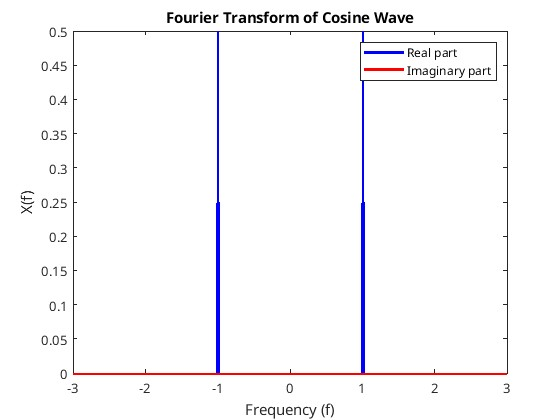
\includegraphics[scale=0.5]{../Ex02.jpg}

\end{aufgabe}

\pagebreak
\begin{aufgabe}{} % Exercise 3 ---------------------------------------------------------------------
  Given are two sines according to the following formula: 
  
  \qquad \(x_i(t)=\sin \left(2 \pi f_i t\right) \text {, with } i \in\{1,2\}\) 
  with 
  \qquad \(f_1=1 \mathrm{~Hz}\) and \(f_2=3 \mathrm{~Hz}\).

  All two sines are time delayed by \(\tau=0.1 \mathrm{~s}\) to yield 
  
  \qquad \(y_i(t)=\sin \left(2 \pi f_i(t-0.1)\right)\)
  
  This corresponds to a phase shift. Thus, the delayed sines may also be written as 
  
  \qquad \(y_i(t)=\sin \left(2 \pi f_i t+\phi_i\right)\)
  
  \begin{enumerate}
  \def\labelenumi{\alph{enumi})}
  \item
    We have to calculate the phase shifts \(\phi_i\) for each sine and verify that this corresponds to the ``Shift Theorem''
  \end{enumerate}
  
  \begin{enumerate}
  \def\labelenumi{\arabic{enumi}.}
  \item
    Calculate the phase shifts \(\phi_i\)
  
    \begin{itemize}
    \item
      We know that: 
      
      \qquad \(\sin \left(2 \pi f_i(t-\tau)\right) = \sin \left(2 \pi f_i t+\phi_i\right)\)

    \item
      So: 

      \qquad \(2 \pi f_i(t-\tau) = 2 \pi f_i t+\phi_i\) 
      
      \qquad \(\implies \phi_i= 2 \pi f_i t - 2 \pi f_i t \tau - 2 \pi f_i t = 2 \pi f_i t \tau\)

    \item
      So we get: 
      
      \qquad \(\phi_1=-2 \pi \cdot 1 \cdot 0.1 = - 0.2\pi\) 
      
      \qquad \(\phi_2=-2 \pi \cdot 3 \cdot 0.1 = -0.6\pi\)

    \end{itemize}
  \item
    Verify that this corresponds to the ``Shift Theorem'' of the Fourier Transform
  
    \begin{itemize}
    \item
      We use the formula for the ``Shift Theorem'' (DSP\_2.pdf, page 41) 
      
      \qquad \(x(t-T)\) \(\circ-\bullet\) \(X(f) e^{-j 2 \pi f T}\)

    \item
      So, since \(\phi_i= 2 \pi f_i t \tau\), we get 
      
      \qquad \(x(t-\tau)\) \(\circ-\bullet\) \(X(f) e^{-j 2 \pi f \tau} = X(f) e^{-j\phi_i}\) q.e.d

    \end{itemize}
  \end{enumerate}
  
  \begin{enumerate}
  \def\labelenumi{\alph{enumi})}
  \setcounter{enumi}{1}
  \item
    For both sines in separated plots: Plot the original signal, the time delayed signal and the phase shifted signal. Since the latter two are identical, show this by plotting the first with a solid line and the overlaid one in a different colour with a dashed line. Plot each signal from 0 to 1s. In Matlab use the following time-vector: \(t=0: 0.001: 1\).
  \end{enumerate}
  
  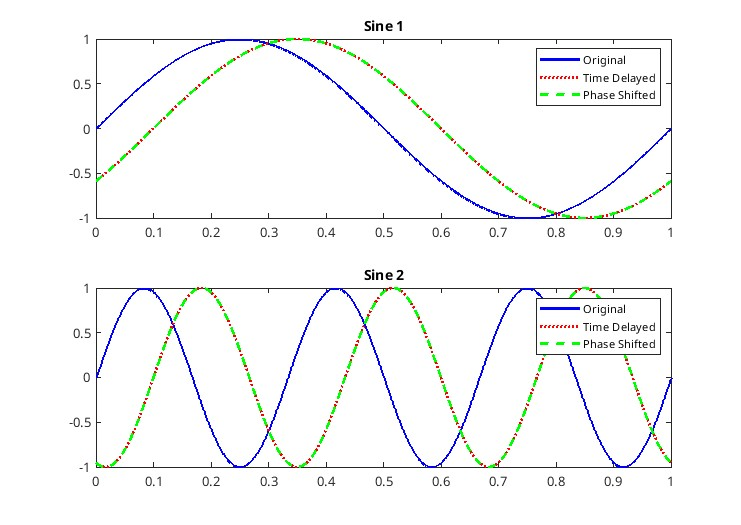
\includegraphics[scale=0.5]{../Ex03.jpg}
\end{aufgabe}

\pagebreak
\begin{aufgabe}{} % Exercise 4 --------------------------------------------------------------------
  We need to find out whether
  \begin{align*}
    &\text{a)} \ y(t) = \left( x(t) \right)^2
    &&\text{b)} \ y(t) = x(t) \cdot \sin{(\Omega_0 t)}
  \end{align*}
  are linear and time invariant.

  \begin{enumerate}
    \item Let $y(t) = \left( x(t) \right)^2$.
    \begin{enumerate}

      \item \textbf{Linearity.} It is easy to see that \underline{the system is not linear}:
      $$
      \left( \alpha x(t) \right)^2
      = \alpha^2 \left( x(t) \right)^2
      = \alpha^2 y(t)
      \neq \alpha y(t).
      $$

      \item \textbf{Time invariance.} Let $y_1(t) = \left( x(t-\tau) \right)^2$ be the system in which input is delayed, and let $y_2(t) = y(t-\tau)$ be the system in which the output is delayed. Since $y_1 = \left( x(t-\tau) \right)^2 = y(t-\tau) = y_2$, we can see that \underline{the system is time invariant}.

    \end{enumerate}

    \item Let $y(t) = x(t) \cdot \sin{(\Omega_0 t)}$.
    \begin{enumerate}

      \item \textbf{Linearity.} Let $y_1(t) = \left(\alpha x_1(t) + \beta x_2(t)\right) \sin{(\Omega_0 t)}$, and let $y_2(t) = \alpha x_1(t) \sin{(\Omega_0 t)} + \beta x_2(t) \sin{(\Omega_0 t)}$. Then we can see that
      $$
      y_1(t) = \left(\alpha x_1(t) + \beta x_2(t)\right) \sin{(\Omega_0 t)} = \alpha x_1(t) \sin{(\Omega_0 t)} + \beta x_2(t) \sin{(\Omega_0 t)} = y_2(t).
      $$
      Therefore, \underline{the system is linear}.

      \item \textbf{Time invariance.} Let $y_1(t) = x(t-\tau) \sin{(\Omega_0 t)}$ be the system in which the input is delayed, and let $y_2(t) = y(t-\tau)$ be the system in which the output is delayed. Since $y_1 = x(t-\tau) \sin{(\Omega_0 t)} \neq x(t-\tau) \sin{(\Omega_0 (t-\tau))} = y(t-\tau) = y_2$, we can see that \underline{the system in not time invariant}.
    \end{enumerate}
  \end{enumerate}

\end{aufgabe}

\end{document}
